\documentclass[conference]{IEEEtran}
\IEEEoverridecommandlockouts
% This is a comment, it's not going to show up in the report, but handy dandy for editing ect
\usepackage{cite}
\usepackage{amsmath,amssymb,amsfonts}
\usepackage{algorithmic}
\usepackage{graphicx}
\usepackage{textcomp}
\usepackage{xcolor}
\def\BibTeX{{\rm B\kern-.05em{\sc i\kern-.025em b}\kern-.08em
    T\kern-.1667em\lower.7ex\hbox{E}\kern-.125emX}}

\begin{document}

\title{Predicting Cardiovascular Disease Using Machine Learning: A Data-Driven Approach \\
{\footnotesize COM747 Data Science and Machine Learning}
}

\author{
\IEEEauthorblockN{\textsuperscript{} Joseph Young}
\IEEEauthorblockA{\textit{B01003963}} 
\and
\IEEEauthorblockN{\textsuperscript{} Hephzibah Wilson}
\IEEEauthorblockA{\textit{B00778496}} 
\and
\IEEEauthorblockN{\textsuperscript{} Moeed Ahmed}
\IEEEauthorblockA{\textit{B01009661}} 
\and
\IEEEauthorblockN{\textsuperscript{} Muhammad Arslan Mustafa}
\IEEEauthorblockA{\textit{B01006361}}
}

\maketitle

\begin{abstract}
Cardiovascular disease (CVD) is a leading global cause of morbidity and mortality, creating a critical need for early detection and prevention. This study applies machine learning techniques to develop a predictive model to identify patients at risk of CVD using an open-source Kaggle dataset containing medical and lifestyle-related attributes including age, gender, blood pressure, cholesterol, glucose levels and life-style factors.

A comprehensive data science pipeline was implemented, handling data cleaning and transformation, feature engineering, and categorical encoding. Exploratory data analysis (EDA) provided insights into potential risk factors. Logistic regression, random forest and k-NN models were evaluated using accuracy, sensitivity, specificity, F1-score and ROC-AUC.

Results demonstrate that data-driven methods can effectively classify individuals at risk of CVD, with Logistic Regression yielding the highest performance. Ethical and professional considerations are addressed emphasizing fairness, transparency, and the potential impact of misclassifications.

This work highlights the value of interpretable machine learning tools in supporting clinical decision-making and public health interventions aimed at reducing cardiovascular risk. 
\end{abstract}
% If have enough words left it might be worth integrating the idea of following CRISP-DM
\section{Introduction}
Cardiovascular disease (CVD) is the leading global cause of death, responsible for approximately 17.9 million deaths annually, according to the World Health Organisation \cite{WHO}. These conditions include coronary artery disease, heart failure, and stroke. Early identification of high-risk individuals is critical for enabling timely interventions and reducing mortality.

Machine learning (ML) is increasingly used in healthcare to uncover complex patterns in medical data. Several studies have demonstrated its effectiveness in predicting CVD using structured health records and open-source datasets \cite{RW1}–\cite{RW3}.

Building upon this research, our project applies a complete data science pipeline to an open Kaggle dataset \cite{DATA}, comprising 70,000 medical records with demographic, biometric, and lifestyle features. We carried out data cleaning, feature engineering, exploratory data analysis (EDA), and trained multiple machine learning models including Logistic Regression, K-Nearest Neighbors, and Random Forest to evaluate their performance in predicting the presence of CVD.


\subsection{Related Works}
Extensive research has investigated CVD risk factors and the use of ML for prediction. Zhang et al.~\cite{ALCOCVD} examined how lifestyle factors like alcohol, BMI, and smoking influence CVD mortality in hypertensive patients. While moderate alcohol intake showed limited protective effects, heavy drinking negated any benefits.

Several studies applied ML techniques to predict CVD. Subramani et al.~\cite{RW1} and Hossain et al.~\cite{RW2} compared models including logistic regression, SVM, random forest, and naive Bayes. Subramani found logistic regression and SVM most effective, highlighting age as the key risk factor. Hossain found random forest performed best, identifying cholesterol as most significant. Both studies were affected by slight class imbalances.

Baghdadi et al.~\cite{RW3} extended prior research by using advanced models and feature selection. CatBoost achieved the best performance, outperforming traditional algorithms like random forest. Age, cholesterol, and blood pressure were found to be significant predictors, though missing data limited the inclusion of some variables.

Overall, these studies demonstrate that ML models can effectively predict CVD risk, though the most suitable model and features may vary by dataset and population.




\subsection{Aim and Objectives}
The primary aim of this project is to develop and evaluate machine learning models that can accurately predict the presence of cardiovascular disease (CVD) using clinical and lifestyle-related data. By leveraging an open-source dataset and applying modern data science techniques, the study seeks to explore how data-driven approaches can assist in early detection and risk stratification of CVD in a general population. 
To achieve this aim, the following objectives were defined:
\begin{enumerate}
    \item To preprocess and clean the dataset by handling outliers, correcting data types, removing duplicates, and engineering new features to enhance model interpretability.
    \item To perform exploratory data analysis (EDA) to identify trends, correlations, and patterns in the dataset relevant to CVD risk.
    \item To implement and compare multiple machine learning classification models, including logistic regression, K-NN and random forest, for predicting cardiovascular disease. 
    \item To evaluate model performance using standard classification metrics such as accuracy, sensitivity, specificity, F1-score, and ROC-AUC.
    \item To reflect on the legal, ethical, and professional considerations in applying machine learning to medical data, with particular attention to data privacy, fairness, and transparency. 
\end{enumerate}
These objectives guided the end-to-end structure of the project, from data acquisition through to evaluation and discussion of results. 

\section{Methods}
\subsection{Data Cleaning and Preprocessing}
The project began with Kaggle’s cardiovascular disease dataset \cite{DATA}, comprising 70,000 anonymised records with 13 clinical and lifestyle features.

The data was imported into R using \texttt{read.csv()} with semicolon delimiters. Key libraries (e.g., \texttt{dplyr}, \texttt{ggplot2}, \texttt{caret}) were loaded via a utility function to ensure reproducibility.

Initial inspection using \texttt{str()}, \texttt{summary()}, and \texttt{colSums(is.na())} confirmed no missing values. Early plots and a correlation matrix revealed key relationships, including positive correlations between age and CVD, weight and CVD, and strong links between cholesterol and glucose.


To enhance data quality, outliers in height, weight, and blood pressure were removed based on realistic ranges. Duplicate rows were also excluded. A new variable, \texttt{age\_years}, was derived by converting age from days to years using \texttt{floor()}, and BMI was calculated.

Categorical variables (e.g., cholesterol, glucose, activity) were converted to factors for proper handling during modeling.

The cleaned dataset was saved as \texttt{cardio\_cleaned.csv}, serving as the foundation for further EDA and model development.


\subsection{Exploratory Data Analysis}

Exploratory Data Analysis (EDA) was conducted on the cleaned dataset to identify key patterns, trends, and relationships that may contribute to the development of predictive models for cardiovascular disease. The analysis explored demographic, biometric, and lifestyle-related features through a series of visualizations and correlation assessments.
A strong focus was placed on investigating correlations between the target variable (cardio) and potential predictors. Among the most notable relationships was the positive correlation between age and disease presence. The majority of diagnosed cases were concentrated in older age groups, particularly between 50 and 65 years as shown in figure 1, which is consistent with well-established clinical understanding that cardiovascular risk increases with age. 

\begin{figure}[htbp]
\centerline{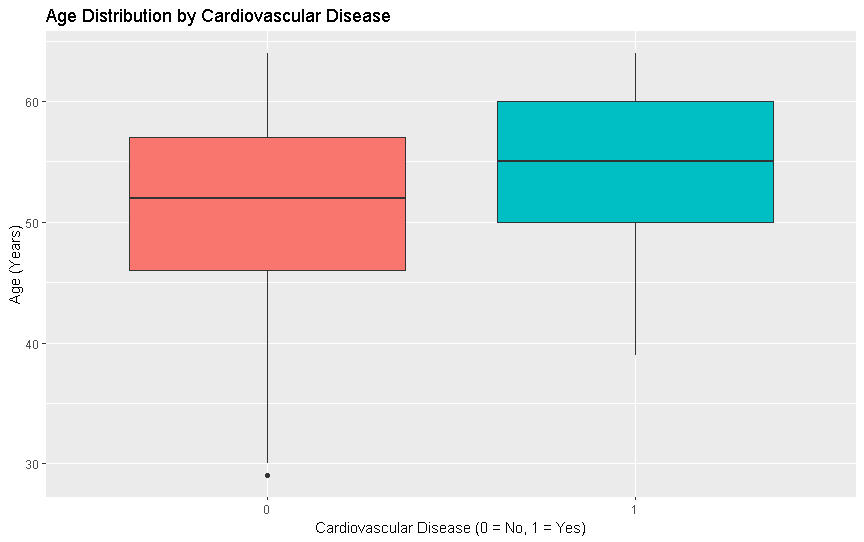
\includegraphics[scale=0.4]{Age Distribution by Cardiovascular Disease.png}}
\caption{Age by CVD Boxplot}
\label{fig}
\end{figure}

Another key finding was the relationship between BMI and cardiovascular disease. Patients with a higher BMI exhibited a noticeably increased likelihood of being diagnosed with CVD. This trend reinforces the link between excess body weight and cardiovascular risk, and supports BMI as a valuable feature for inclusion in predictive modeling.
Elevated cholesterol and glucose levels were also associated with a higher incidence of CVD. Although these variables showed only moderate correlation with the target, their clinical significance justifies their inclusion in the model. Interestingly, while cholesterol levels were generally higher among female patients, the proportion of CVD cases was slightly greater in males, suggesting that gender may play a role in how these risk factors manifest.

The analysis of lifestyle variables, such as smoking and alcohol consumption, revealed they were more common among male patients. However, these variables did not show a strong direct correlation with CVD in this dataset. This could be due to underreporting, dataset limitations, or the fact that their impact may be more nuanced when interacting with other factors like age or BMI. % We could mention that this is contrary to what is currently known and find reference HEPHZI

Correlations among numeric features were visualized using a heatmap as shown in Figure 2. As expected, a strong relationship was observed between systolic and diastolic blood pressure, and between weight and BMI. These redundancies and overlaps were taken into account for feature selection to avoid multicollinearity in some models. 

\begin{figure}[htbp]
\centerline{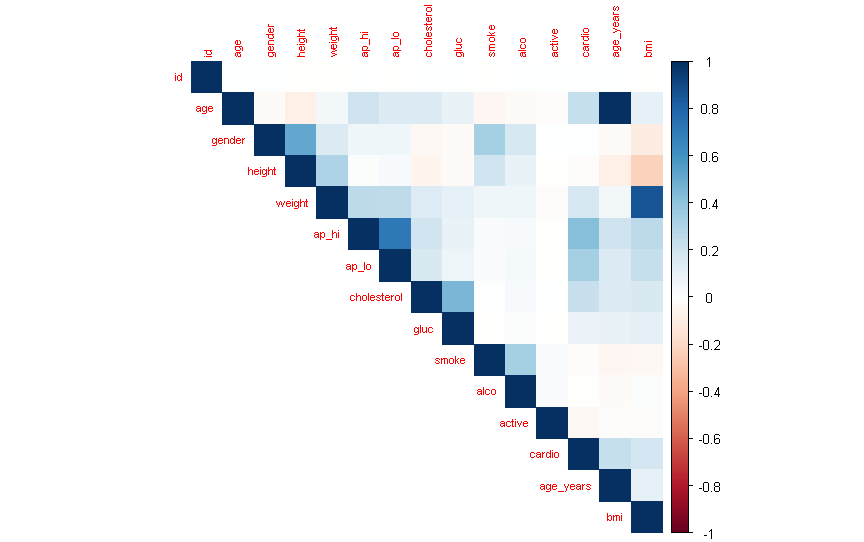
\includegraphics[scale=0.4]{Correlation matrix for numeric variables.png}}
\caption{Correlation matrix for numeric Variables}
\label{fig}
\end{figure}

Overall, the EDA phase provided valuable insights that guiding the selection and transformation of features of modeling. The observed relationships helped validate medical assumptions and highlighted which variables may have stronger predictive power. These findings informed decisions on feature engineering, model input design, and considerations for ensuring fairness and generalisability across gender and age subgroups. 

\subsection{Feature Engineering} 

Feature engineering was implemented to improve the quality, interpretability, and predictive power of the input data for the models' development.

An id column which served no predictive purpose and was removed. Numerical features (age\_years, height, weight, systolic blood pressure (ap\_hi), diastolic blood pressure (ap\_lo), and BMI) Z-score normalized to ensure that features were on a consistent scale, important for distance-based models and algorithms sensitive to feature magnitude.

Categorical variables (cholesterol and glucose level)  were transformed into factors with meaningful labels: "normal", "above\_normal", and "well\_above\_normal" to improve interpretability and model readiness and then one-hot encoded using dummy variable creation. This avoids unintended ordinal interpretation and allows models to treat each level as an independent feature. These dummy variables were appended to the dataset while the original factor variables were removed. 

The target variable cardio was converted to a binary format (No/Yes) for binary classification. The fully preprocessed dataset was saved as cardio\_model\_ready.csv, for all subsequent modelling.

Feature engineering ensured a clean, well-structured dataset, compatible with various machine learning algorithms while reducing potential bias from improperly scaled or misinterpreted features. 

\subsection{Data Splitting}
To ensure that all models were comparable with each other, a data splitting phase was added.
A seed was set which ensured that the split was reproducible between different runs. 

The dataset was partitioned using Caret's createDataPartition function, with cardio as the target feature. This split the data in a stratified manner and randomly sampled from each class (those with CVD and those without) until the desired proportions are achieved \cite{DATAPART}.

Seventy percent of the cleaned and feature engineered dataset was allocated for training, and the remaining thirty percent was reserved for testing, therefore reducing the risk of overfitting.
The proportion of patients with and without CVD in each group was verified to ensure the datasets were balanced. Once validated, the datasets were saved in separate CSV files for model development and evaluation. 

\subsection{Logistic Regression Model}
% HEPHZI Don't talk about results, just training, creation and how results were achieved
% Why it was chosen ADD REFERENCE HERE!!!
The initial model considered was a Logistic Regression Model. As disease diagnosis is a binary classification problem, it was a natural fit. Logistic Regression allows both probability prediction based upon the risk factors and feature importance analysis. Other studies investigating ML methods for CVD classification have found LR to achieve higher accuracy than other models \cite{OTHERLOGREG}, as disc
used in related works.
% Creation and training

The model was implemented using the glm function with a family of "binomial(link="logit")" and a target of "cardio \~ ." to specify that the model should be a logistic regression model that predicts the probability that a patient suffers from CVD. The training utilized the dataset created in the previous section.
% Making predictions

Testing was performed using the predict function upon the testing dataset, creating probabilities between 0 and 1. These were also converted to binary classifications for evaluation. 
% Confusion matrix
% AUC and ROC
% Regression Curves, F1 ect

Several metrics were used for model evaluation. A confusion matrix function from Caret provided values for accuracy, F1 score, sensitivity and specificity. A ROC curve was plotted using pROC and ggplot2. The AUC (Area under the Curve) was calculated to evaluate the prediction of true positives and false positives. To interpret feature importance, logistic curves and barcharts were created and the odds ratios for each feature was calculated. Figure 3 shows ap-hi's regression curve. 

\begin{figure}[htbp]
\centerline{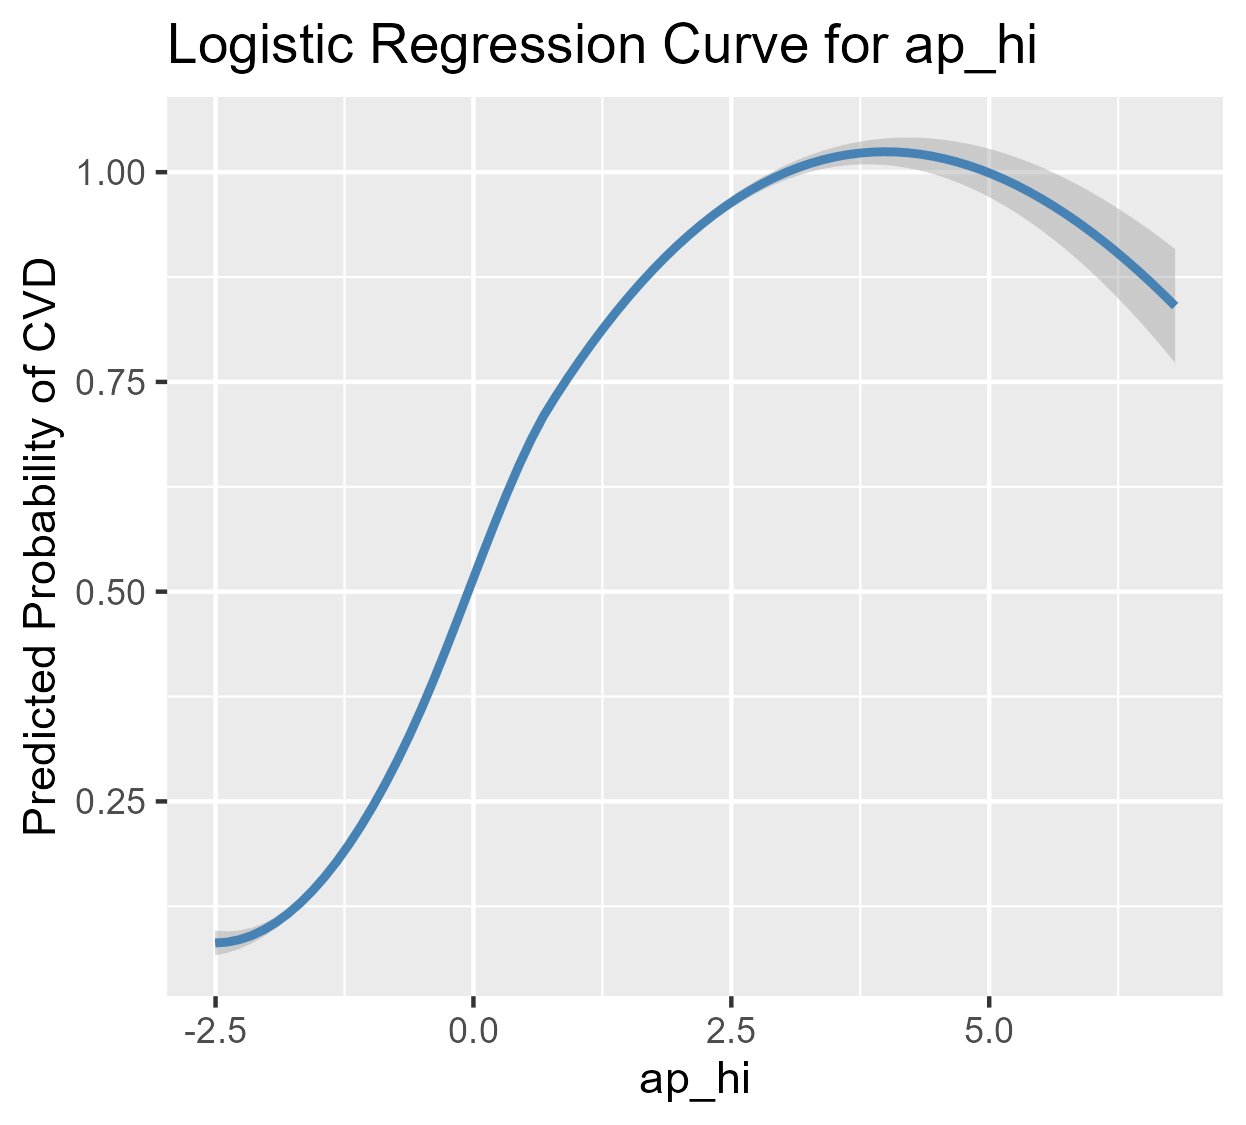
\includegraphics[scale=0.5]{cvdByap_hiLC.png}}
\caption{Logistic Regression Curve for ap-hi}
\label{fig}
\end{figure}

% Saving model
Finally, the model was saved as an RDS file for future reference. 

\subsection{K-NN Model}
%Diseases of the heart have been among the leading causes of death across the globe in the latest years. It is extremely necessary to detect such diseases at an early stage in order to reduce the risk of severe complications and enable timely medical intervention. Due to the high rise in healthcare information, machine learning algorithms have proved to be of great assistance in reviewing patient data and making predictions on disease risk such as in the case of heart disease. For this research, the K-Nearest Neighbors (KNN) algorithm was applied in classifying whether or not a patient would develop heart disease based on structured and prepared clinical information.

% Need to make more concise - H
The K-Nearest Neighbors (K-NN) algorithm was applied to predict probability of CVD. KNN was utilized because it does not require pre-defined rules but makes predictions based upon neighboring data points in the feature space, and it is simple to implement and interpret, all of which makes it a good fit for multidimensional medical data. 

Research by M.A. Jabbar et al \cite{KNN} established K-NN's suitability for CVD prediction, provided that the data is preprocessed correctly and features are appropriately chosen. These methodologies were applied in this project. 

The K-NN model was created using the train() function from the caret package, applying 10-fold cross-validation. Preprocessing operations included centering and scaling to normalize the numeric variables. This aided in the computation of the distance between the observations precisely. The predict() function was utilized to obtain class labels and predictions on the test data.

Evaluation metrics were generated using the confusionMatrix() function including accuracy, sensitivity, specificity, and F1 score. An ROC curve was generated with the ggroc() function of the pROC package. The AUC was computed with the auc() function to understand how accurately the model would be able to distinguish between different classes. Ggplot2 was used to visualise the connections between predicted values and variables such as BMI and gender.

%Applying KNN in the research paid off for forecasting the risk of heart disease. Patient data were utilized in the model as well as an effective means of classifying information, yielding consistent outcomes and enabling doctors to make informed decisions as well as avoid health issues.

\subsection{Random Forest Model}
Several studies have validated the effectiveness of Random Forest models for predicting CVD risk. Guadadhe et al. \cite{RF1} and Dinh et al. \cite{RF2} found that Random forest outperformed other models, while Krittanawong et al. \cite{RF3} highlighted that ensemble models like Random Forest are more adaptable to complex interactions within electronic health records. 

Random Forest builds multiple decision trees and combines their outputs to improve accuracy and reduce overfitting. It handles both numerical and categorical features well, is robust to noise and missing values, and allows feature importance to be measured.

The model was trained with the split training data and using the randomForest package with 100 trees. The model was saved with saveRDS for reuse and further examination. Predictions were made on the test dataset using the predict function to get both classes and probabilities. This allowed for model validation.

Evaluation metrics were generated using the confusionMatrix function, providing the confusion matrix, accuracy, sensitivity, specificity and F1 values. An ROC curve was plotted and the AUC calculated to assess model performance. Feature importance was visualised using the varImpPlot function and bootstrap confidence intervals for predicted probabilities were generated using a t-test.


\section{Results}
% Will argue that logistic regression is the best model, despite lower specificity due to nature of CVD diagnosis. Would rather a false positive (higher sensitivity) which would lead to investigation rather than false negative (higher specificity) which could result in a failure to treat illness. 
% Need to explain why each metric was used, it's also possible a test should be run to compare them
% Show graph of all rocs, compare f1 scores, bit about expected outcomes vs actual
\begin{table}[]
\caption{Model Evaluation Metrics}
\begin{tabular}{llllll}
Model               & Accuracy & Specificity & Sensitivity & F1 Score & ROC AUC \\
LR & 0.7279   & 0.6670      & 0.7873      & 0.7457   & 0.7897  \\
K-NN                & 0.7082   & 0.6799      & 0.7367      & 0.7186   & 0.7629  \\
RF       & 0.7237   & 0.6888      & 0.7576      & 0.7353   & 0.7857
\end{tabular}
\end{table}

This section compares the three created models: Logistic Regression, K-NN and Random forest.
Table 1 displays the metrics gathered for evaluation, while fig 1 shows a comparison of the ROC for each model.

All models successfully predicted CVD in most cases, achieving similar accuracies. Logistic regression performed best overall with the highest accuracy (0.7279), F1 score (0.7457) and ROC-AUC (0.7897), however it had the lowest specificity. This shows strong ability in predicting those with CVD, but weakness predicting the absence of CVD. Blood pressure (ap-hi) had the greatest feature importance with the lowest p-value. %Would like something critical here, predicting too many positives which results in poorer performance of negatives

Random Forest performed similarly with marginally poorer metrics, however had slightly better specificity (0.6888). It too found that ap-hi had greatest feature importance using the varImpPlot() function.

K-NN had the poorest performance overall, though its specificity (0.6799) surpassed logistic regression. It also identified that ap-hi was the greatest predictor with the varImp() function.

Logistic Regression was selected as the optimal choice due to its superior performance, and the medical context. For CVD risk prediction, greater sensitivity was prioritised over greater specificity as false positives are investigated further, however false negatives may delay treatment. All three models identified that high blood pressure (ap-hi) was the greatest risk factor.



\begin{figure}[htbp]
\centerline{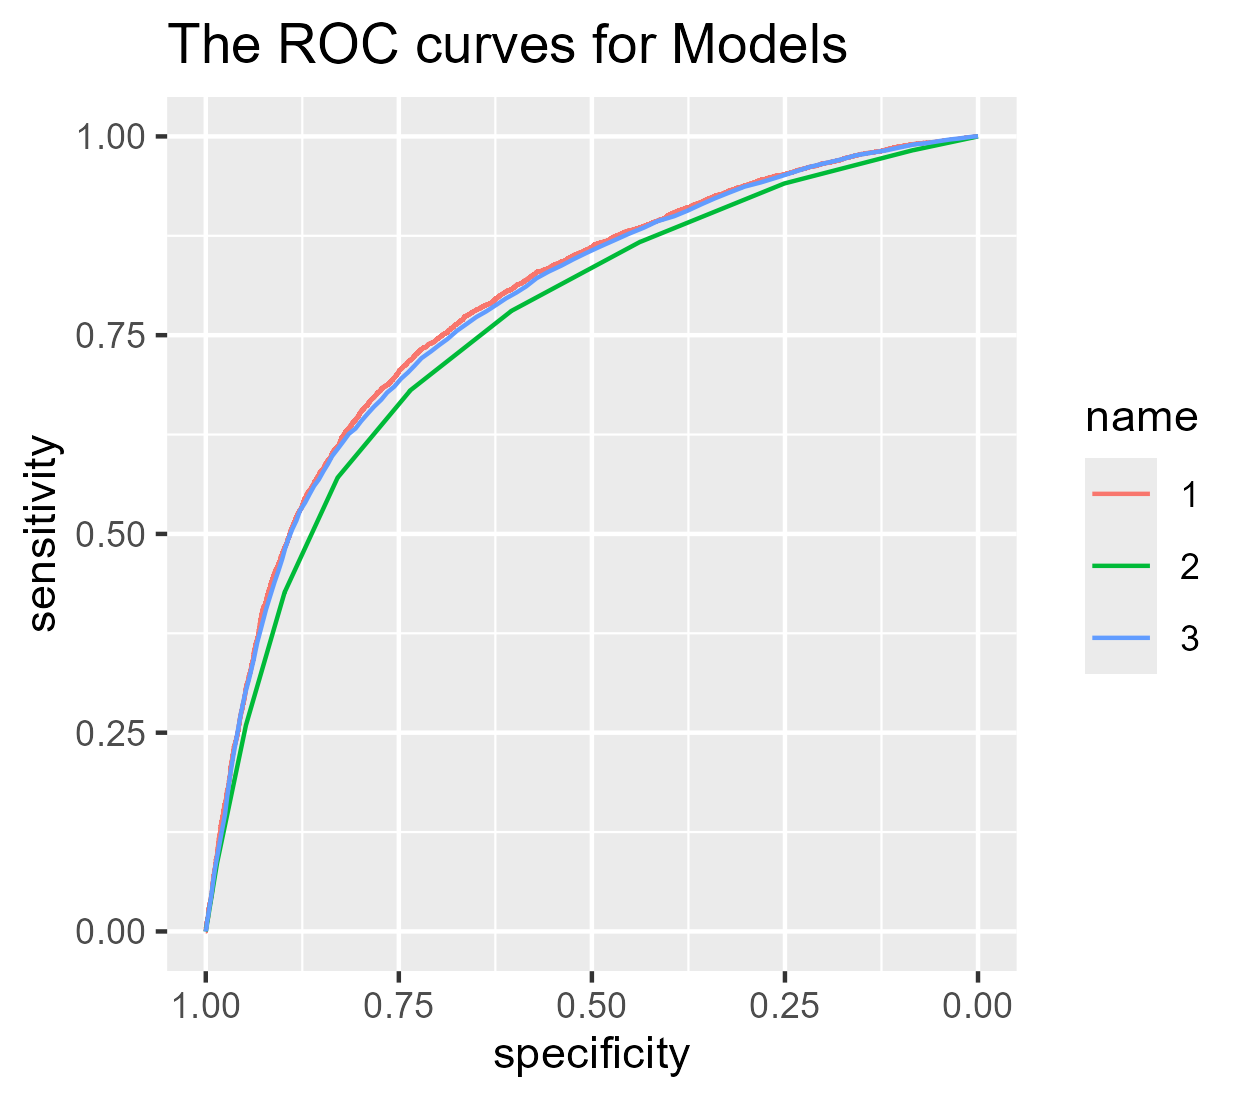
\includegraphics[scale=0.5]{all_rocs_plot.png}}
\caption{1: LR, 2: K-NN, 3:RF}
\label{fig}
\end{figure}

\section{Discussion}
\subsection{Limitations} % Need to make more concise
Despite achieving reasonable accuracy across all three models, there were some limitations.
% Generalisation - Dataset likely taken from a localised population (same healthcare system) therefore other populations may differ.
The dataset likely represents a single healthcare system and localized population and, as explored earlier, different populations can vary in the most significant risk factors. Therefore the models may have limited generalisability. Integrating data from multiple healthcare systems could improve this.
% Missing information - No metric for family history, medication ect, so missing potentially significant factors
Some potentially significant missing factors were missing from the dataset including family history of heart disease, medications use and comorbidities, the inclusion of which may have resulted in stronger accuracy.
% Social imbalance - No socioeconomic or racial factors - Difficult to access fairness or bias/ more vulnerable populations
The lack of socioeconomic or information about ethnicity, makes it difficult to assess the fairness or bias when considering vulnerable or disadvantaged populations.
% Lack of temporal data - Data from one snapshot in time, more accurate modeling could occur if had information over a period of time
The dataset used only showed information from one snapshot in time. As Zhange et al \cite{RW1} demonstrated, risk factors can manifest differently over time, therefore with temporal data, the models could more accurately interpret risk.
% Gender imbalance - Unsure if women are more likely to conduct a medical census
Gender imbalance, with a majority of patients being women could have limited the accuracy of the models as risk factors that have a greater impact on women could be overrepresented in our final models.
\subsection{Ethical Considerations}
Due to the sensitive nature of the subject, it was particularly important to consider ethical factors throughout the development of the project.
\subsubsection{Sustainability}
To ensure maintainability and updatability, a Git repository was created and hosted remotely on GitHub which allowed for collaborative access to the project \cite{GIT}. A single, well documented script was used for the entire pipeline which prevented redundant code and improved clarity. Random seeds were set to ensure reproducability of data sets and models and all created datasets and models were saved to the results directory. 
\subsubsection{Data Reliability}
Several risk factors in the dataset were self-reported (alcohol intake, smoking and activity), potentially reducing reliability due to human biases that may have led to over or under reporting. Activity in particular raised potential issues as no threshold was given for what constitutes an active person. Despite it's subjective nature, it was decided that it was still a useful metric. 
\subsubsection{Inclusivity} %Check out my semi colon here! :)
As age is a significant risk factor for CVD, a wide range of ages were represented as clarified using histogram visualisations (see figure 4). Similarly to many other medical datasets, the gender distribution was skewed\cite{GENDER}; approximately 65\% of patients in the dataset were female. To mitigate any bias, EDA explored the differences between risk factors between genders, and the proportion of CVD in each gender was verified to be approximately equal. Ethnicity was not included as a factor in this dataset, which limits the models as certain CVD conditions disproportionately affect specific ethnic groups \cite{ETHNICITY}. 
\begin{figure}[htbp]
\centerline{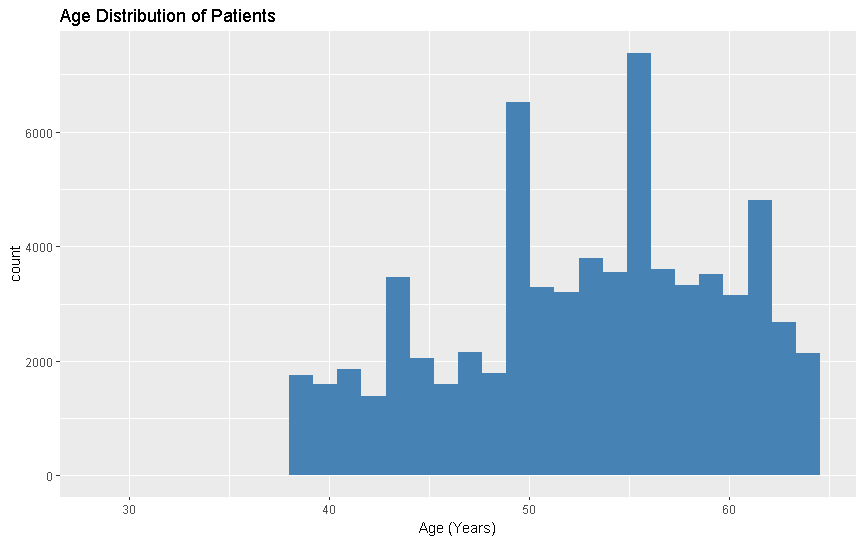
\includegraphics[scale=0.25]{Age Distribution of Patients.png}}
\caption{Age distribution of Patients}
\label{fig}
\end{figure}

% Trustworthiness of Created AI systems - Verifying data, overfitting
\subsubsection{Trustworthiness}
To increase model trustworthiness, data cleansing removed outliers that could skew results, duplicate rows and checked for any missing values. To minimize the risk of overfitting, a comprehensive dataset (70,000 rows) was chosen, and before training, the data was split randomly into training and testing to ensure the models could handle unseen data. Performance metrics were chosen to verify the quality of each model.
% Legality - Data protection, GDPR, Open data
\subsubsection{Legality}
To comply with GDPR (General Protection Regulation) standards \cite{GDPR}, an open source, fully anonymised dataset was chosen where patients could only be identified through a ID number. This is particularly important in medical contexts due to the sensitive nature of the data. In future synthetic data could be generated using SMOTE (Synthetic Minority Over-sampling Technique) or Synthpop while simultaneously addressing class imbalances. 
% Social - Impact of this tech? Like could be used to screen potential patients at risk, good, if replace doctors bad?
\subsubsection{Social Impact}
AI tool for CVD risk assessment has the potential for positive and negative social effects. Previously undetected risk factors may be identified enabling early interventions. However, as no model was 100\% accurate, false positive and negatives are inevitable which may result in unnecessary treatment, or patients being unable to receive the necessary care. To reduce risk, sensitivity was prioritised over specificity to minimize the number of missed cases, and in practice would function to aid decision making by qualified doctors. 

\section{Conclusion}
This study demonstrated the effectiveness of machine learning in predicting cardiovascular disease using structured health data. By developing a complete data pipeline and evaluating multiple models, we found that logistic regression offered the best balance of accuracy and interpretability - making it well-suited for clinical use where sensitivity is critical.

Key risk factors such as age, blood pressure, and BMI were consistent with clinical expectations, supporting the model's relevance. While limitations exist, such as the lack of temporal or demographic diversity, this work shows the potential of data-driven approach to support early diagnosis and improve public health outcomes.





% There is a handier way to do this, but I can't for the life of me remember how. Probably just best to use a IEEE reference generator to get the formatting right and copy and paste them in. These are just the built in examples
\begin{thebibliography}{00}
\bibitem{WHO} WHO, “Cardiovascular Diseases (CVDs),” World Health Organization, Jun. 11, 2021. https://www.who.int/news-room/fact-sheets/detail/cardiovascular-diseases-(cvds)
\bibitem{RW1} [S. Subramani et al., "Cardiovascular diseases prediction by machine learning incorporation with deep learning," *Frontiers in Medicine*, vol. 10, 2023. [Online]. Available: https://www.frontiersin.org/journals/medicine/articles/10.3389/fmed.2023.1150933/full
\bibitem{RW2} S.Hossain et al. , "Machine learning approach for predicting cardiovascular disease in Bangladesh: evidence from a cross-sectional study in 2023" *BMC Cardiovascular Disorders*, vol. 24, no.1, 2024. [Online]. Available: https://bmccardiovascdisord.biomedcentral.com/articles/10.1186/s12872-024-03883-2 
\bibitem{RW3} N. A. Baghdadi et al., "Advanced machine learning techniques for cardiovascular disease early detection and diagnosis" *Journal of Big Data*, vol. 10, 2023. [Online]. Available: https://journalofbigdata.springeropen.com/articles/10.1186/s40537-023-00817-1
\bibitem{ALCOCVD} Z. Yu-Jun et al., “Alcohol drinking triggered decrease of oxidative balance score is associated with high all-cause and cardiovascular mortality in hypertensive individuals: findings from NHANES 1999– 2014,” Journal of Geriatric Cardiology, vol. 21, no. 8, pp. 779–790, 2024, Available: https://research.ebsco.com/linkprocessor/plink?id=f26d2ce7-665f-3de6-b9b4-ede8774f74d7
\bibitem{DATA} D. Sulianova, "Cardiovascular Disease Dataset," Kaggle. [Online]. Available: https://www.kaggle.com/datasets/sulianova/cardiovascular-disease-dataset
\bibitem{DATAPART} “createDataPartition function - RDocumentation,” Rdocumentation.org, 2024. https://www.rdocumentation.org/packages/caret/versions/7.0-1/topics/createDataPartition.
\bibitem{GIT} J. Young, H. Wilson, M. Ahmed, and M. A. Mustafa, “GitHub - jyoung56/com747Group13: Group Assignment for COM747 Data Science and Machine Learning,” GitHub, 2025. https://github.com/jyoung56/com747Group13
\bibitem{OTHERLOGREG}Y. Boer, L. Valencia, M. R. Setiadi, K. Eka Setiawan and M. F. Hasani, "Classification of Heart Disease: Comparative Analysis using KNN, Random Forest, Gaussian Naive Bayes, XGBoost, SVM, Decision Tree, and Logistic Regression," in 2023 5th International Conference on Cybernetics and Intelligent System (ICORIS), Pangkalpinang, Indonesia, 2023, pp. 1-5
\bibitem{KNN} M. A. Jabbar, B. L. Deekshatulu, and P. Chandra, “Heart Disease Prediction System using K-Nearest Neighbor Algorithm,” Procedia Computer Science, vol. 85, pp. 135–142, 2016, doi: 10.1016/j.procs.2016.05.204.
\bibitem{RF1} M. Gudadhe, K. Wankhade and S. Dongre, "Decision support system for heart disease based on support vector machine and Artificial Neural Network," 2010 International Conference on Computer and Communication Technology (ICCCT), Allahabad, India, 2010, pp. 741-745, doi: 10.1109 ICCCT.2010.5640377
\bibitem{RF2} A. Dinh, S. Miertschin, A. Young, and S. D. Mohanty, “A data-driven approach to predicting diabetes and cardiovascular disease with machine learning,” BMC Medical Informatics and Decision Making, vol. 19, no. 1, Nov. 2019, doi: https://doi.org/10.1186/s12911-019-0918-5.
\bibitem{RF3} C. Krittanawong, H. Zhang, Z. Wang, M. Aydar, and T. Kitai, “Artificial Intelligence in Precision Cardiovascular Medicine,” Journal of the American College of Cardiology, vol. 69, no. 21, pp. 2657–2664, May 2017, Available: https://www.sciencedirect.com/science/article/pii/S0735109717368456
\bibitem{GENDER} J. Plevkova et al., "Various Aspects of Sex and Gender Bias in Biomedical Research," Physiological Research, vol. 69, pp. S367–S378, 2020
\bibitem{ETHNICITY} A. K. Kurian and K. M. Cardarelli, "Racial and ethnic differences in cardiovascular disease risk factors." Ethnicity \& Disease, vol. 17, no. 1, pp. 143–152, 2007.
\bibitem{GDPR} M. Schulz and J. A. Hennis-Plasschaert, Regulation (EU) 2016/679 of the European Parliament and of the Council of 27 April 2016 on the protection of natural persons with regard to the processing of personal data and on the free movement of such data (United Kingdom General Data Protection Regulation). 2016. Available: https://www.legislation.gov.uk/eur/2016/679/introduction
\end{thebibliography}


\vspace{12pt}
\color{red}
Word Count, non-inclusive of references: NUMBERS HERE

\end{document}
